\begin{titre}[Géométrie dans l'espace]

\Titre{Calculs et positions relatives}{8}
\end{titre}


\begin{CpsCol}
\textbf{Positions relatives}
\begin{description}
\item[$\square$] Construire un patron d'un solide usuel (parallélépipède rectangle, pyramides, cônes de révolution)
\item[$\square$] Construire avec un logiciel dynamique un solide usuel
\item[$\square$] Représenter en perspective cavalière
\item[$\square$] Visualiser la position relative d'une droite et d'un plan, de deux plans
\item[$\square$] Effectuer des calculs de longueurs, de volumes, d'aires
\end{description}
\end{CpsCol}


\EPCB{1}{GE-0}{Chercher. Représenter.}


\begin{DefT}{Perspective cavalière}\index{Perspective cavalière}
La représentation de solide de l'espace en perspective cavalière respecte les règles suivantes  :
\begin{description}
\item[•] la figure vue de face à les dimensions grandeur réelle (sans changer sa forme : un carré est un carré, un rectangle est un rectangle....) 
\item[•] deux droites parallèles sont représentées par 2 droites parallèles
\item[•] des points alignés sont représentés par des points alignés
\item[•] le milieu d'un segment est représenté par le milieu du segment dessiné
\item[•] les éléments non visibles sont dessinés en pointillés, les éléments visibles en traits pleins
\end{description}
\end{DefT}

\mini{
\EPCC{1}{GE-1}{Chercher. Représenter.}
}{
\EPCC{1}{GE-2}{Chercher. Représenter.}
}

\begin{Reg}[ d'incidence]
\begin{description}
\item[R1] Dans chaque plan de l'espace,on peut appliquer tous les théorèmes de géométrie plane (théorèmes de Pythagore, de Thalès,...).
\item[R2]  Par deux points distincts de l'espace, il passe une unique droite.
\item[R3]  Par trois points non alignes A, B et C de l'espace, il passe un unique plan, noté (ABC)
\item[R4]   Si deux points distincts A et B de l'espace appartiennent à un plan P, alors la droite (AB) est contenue dans le plan P.
\end{description}
\end{Reg}

\mini{
\EPCB{1}{GE-7}{Chercher. Représenter. Calculer.}


}{
\EPCB{1}{GE-9}{Chercher. Représenter. Calculer.}

\EPCB{1}{GE-10}{Chercher. Représenter. Calculer.}
}

\EPCB{1}{GE-8}{Chercher. Représenter. Modéliser. Calculer.}

\begin{Reg}[Positions relatives de deux droites]
\begin{description}
\item[R5]   Deux droites de l'espace sont soit coplanaires, soit non coplanaires.
\end{description}


\begin{tabular}{|>{\centering\arraybackslash}p{3.75cm}|>{\centering\arraybackslash}p{3.75cm}|>{\centering\arraybackslash}p{3.75cm}|>{\centering\arraybackslash}p{3.75cm}|}
\hline 
\multicolumn{3}{|c|}{Droites coplanaires (dans un même plan)} & Droites non coplanaires  \\ 
\hline 
d et d' sécantes & \multicolumn{2}{c|}{d et d' parallèles} &  \\ 
\hline 
\definecolor{ffqqqq}{rgb}{1.,0.,0.}
\definecolor{qqqqff}{rgb}{0.,0.,1.}
\begin{tikzpicture}[line cap=round,line join=round,>=triangle 45,x=0.7cm,y=0.7cm].0cm]
\clip(-8.22,-3.62) rectangle (-2.46,1.82);
\draw [color=qqqqff] (-7.,-3.)-- (-4.,-3.);
\draw [color=qqqqff] (-4.,-3.)-- (-3.,-2.);
\draw [dash pattern=on 2pt off 2pt,color=qqqqff] (-3.,-2.)-- (-6.,-2.);
\draw [dash pattern=on 2pt off 2pt,color=qqqqff] (-6.,-2.)-- (-7.,-3.);
\draw [color=qqqqff] (-7.,0.)-- (-4.,0.);
\draw [color=qqqqff] (-4.,0.)-- (-3.,1.);
\draw [color=qqqqff] (-3.,1.)-- (-6.,1.);
\draw [color=qqqqff] (-6.,1.)-- (-7.,0.);
\draw [color=qqqqff] (-7.,0.)-- (-7.,-3.);
\draw [color=qqqqff] (-4.,0.)-- (-4.,-3.);
\draw [color=qqqqff] (-3.,1.)-- (-3.,-2.);
\draw [dash pattern=on 2pt off 2pt,color=qqqqff] (-6.,1.)-- (-6.,-2.);
\draw [color=ffqqqq,domain=-8.22:-2.66] plot(\x,{(-9.-0.*\x)/3.});
\draw [dash pattern=on 2pt off 2pt, color=ffqqqq,domain=-8.22:-2.46] plot(\x,{(-5.25--0.75*\x)/3.75});
\draw [color=ffqqqq,domain=-8.22:-6.86] plot(\x,{(-5.25--0.75*\x)/3.75});
\draw [color=ffqqqq,domain=-3.02:-2.66] plot(\x,{(-5.25--0.75*\x)/3.75});
\begin{scriptsize}
\draw [color=qqqqff] (-7.,-3.)-- ++(-2.5pt,0 pt) -- ++(5.0pt,0 pt) ++(-2.5pt,-2.5pt) -- ++(0 pt,5.0pt);
\draw[color=qqqqff] (-7.34,-2.76) node {$A$};
\draw [color=qqqqff] (-4.,-3.)-- ++(-2.5pt,0 pt) -- ++(5.0pt,0 pt) ++(-2.5pt,-2.5pt) -- ++(0 pt,5.0pt);
\draw[color=qqqqff] (-3.8,-3.1) node {$B$};
\draw [color=qqqqff] (-3.,-2.)-- ++(-2.5pt,0 pt) -- ++(5.0pt,0 pt) ++(-2.5pt,-2.5pt) -- ++(0 pt,5.0pt);
\draw[color=qqqqff] (-2.86,-1.64) node {$C$};
\draw [color=qqqqff] (-6.,-2.)-- ++(-2.5pt,0 pt) -- ++(5.0pt,0 pt) ++(-2.5pt,-2.5pt) -- ++(0 pt,5.0pt);
\draw[color=qqqqff] (-5.78,-1.7) node {$D$};
\draw [color=qqqqff] (-7.,0.)-- ++(-2.5pt,0 pt) -- ++(5.0pt,0 pt) ++(-2.5pt,-2.5pt) -- ++(0 pt,5.0pt);
\draw[color=qqqqff] (-7.24,0.26) node {$E$};
\draw [color=qqqqff] (-4.,0.)-- ++(-2.5pt,0 pt) -- ++(5.0pt,0 pt) ++(-2.5pt,-2.5pt) -- ++(0 pt,5.0pt);
\draw[color=qqqqff] (-3.82,-0.2) node {$F$};
\draw [color=qqqqff] (-3.,1.)-- ++(-2.5pt,0 pt) -- ++(5.0pt,0 pt) ++(-2.5pt,-2.5pt) -- ++(0 pt,5.0pt);
\draw[color=qqqqff] (-2.86,1.36) node {$G$};
\draw [color=qqqqff] (-6.,1.)-- ++(-2.5pt,0 pt) -- ++(5.0pt,0 pt) ++(-2.5pt,-2.5pt) -- ++(0 pt,5.0pt);
\draw[color=qqqqff] (-5.86,1.36) node {$H$};
\draw[color=ffqqqq] (-17.32,-2.68) node {$s$};
\draw [fill=black] (-6.75,-2.75) circle (1pt);
\draw[color=black] (-6.6,-2.4) node {$I$};
\end{scriptsize}
\end{tikzpicture}
  & 
  
\definecolor{ffqqqq}{rgb}{1.,0.,0.}
\definecolor{qqqqff}{rgb}{0.,0.,1.}
\begin{tikzpicture}[line cap=round,line join=round,>=triangle 45,x=0.7cm,y=0.7cm]
\clip(-7.84,-3.56) rectangle (-1.86,2.08);
\draw [color=qqqqff] (-7.,-3.)-- (-4.,-3.);
\draw [color=qqqqff] (-4.,-3.)-- (-3.,-2.);
\draw [dash pattern=on 2pt off 2pt,color=qqqqff] (-3.,-2.)-- (-6.,-2.);
\draw [dash pattern=on 2pt off 2pt,color=qqqqff] (-6.,-2.)-- (-7.,-3.);
\draw [color=qqqqff] (-7.,0.)-- (-4.,0.);
\draw [color=qqqqff] (-4.,0.)-- (-3.,1.);
\draw [color=qqqqff] (-3.,1.)-- (-6.,1.);
\draw [color=qqqqff] (-6.,1.)-- (-7.,0.);
\draw [color=qqqqff] (-7.,0.)-- (-7.,-3.);
\draw [color=qqqqff] (-4.,0.)-- (-4.,-3.);
\draw [color=qqqqff] (-3.,1.)-- (-3.,-2.);
\draw [dash pattern=on 2pt off 2pt,color=qqqqff] (-6.,1.)-- (-6.,-2.);
\draw [color=ffqqqq,domain=-7.84:-2.36] plot(\x,{(-9.-0.*\x)/3.});
\draw [color=ffqqqq,domain=-7.84:-2.36] plot(\x,{(--3.-0.*\x)/3.});
\begin{scriptsize}
\draw [color=qqqqff] (-7.,-3.)-- ++(-2.5pt,0 pt) -- ++(5.0pt,0 pt) ++(-2.5pt,-2.5pt) -- ++(0 pt,5.0pt);
\draw[color=qqqqff] (-7.34,-2.76) node {$A$};
\draw [color=qqqqff] (-4.,-3.)-- ++(-2.5pt,0 pt) -- ++(5.0pt,0 pt) ++(-2.5pt,-2.5pt) -- ++(0 pt,5.0pt);
\draw[color=qqqqff] (-3.8,-3.1) node {$B$};
\draw [color=qqqqff] (-3.,-2.)-- ++(-2.5pt,0 pt) -- ++(5.0pt,0 pt) ++(-2.5pt,-2.5pt) -- ++(0 pt,5.0pt);
\draw[color=qqqqff] (-2.86,-1.64) node {$C$};
\draw [color=qqqqff] (-6.,-2.)-- ++(-2.5pt,0 pt) -- ++(5.0pt,0 pt) ++(-2.5pt,-2.5pt) -- ++(0 pt,5.0pt);
\draw[color=qqqqff] (-5.78,-1.7) node {$D$};
\draw [color=qqqqff] (-7.,0.)-- ++(-2.5pt,0 pt) -- ++(5.0pt,0 pt) ++(-2.5pt,-2.5pt) -- ++(0 pt,5.0pt);
\draw[color=qqqqff] (-7.24,0.26) node {$E$};
\draw [color=qqqqff] (-4.,0.)-- ++(-2.5pt,0 pt) -- ++(5.0pt,0 pt) ++(-2.5pt,-2.5pt) -- ++(0 pt,5.0pt);
\draw[color=qqqqff] (-3.82,-0.2) node {$F$};
\draw [color=qqqqff] (-3.,1.)-- ++(-2.5pt,0 pt) -- ++(5.0pt,0 pt) ++(-2.5pt,-2.5pt) -- ++(0 pt,5.0pt);
\draw[color=qqqqff] (-2.86,1.36) node {$G$};
\draw [color=qqqqff] (-6.,1.)-- ++(-2.5pt,0 pt) -- ++(5.0pt,0 pt) ++(-2.5pt,-2.5pt) -- ++(0 pt,5.0pt);
\draw[color=qqqqff] (-5.86,1.36) node {$H$};
\draw[color=ffqqqq] (-17.32,-2.68) node {$s$};
\draw[color=ffqqqq] (-17.32,0.84) node {$t$};
\end{scriptsize}
\end{tikzpicture}  
  
  
  & 

\definecolor{ffqqqq}{rgb}{1.,0.,0.}
\definecolor{qqqqff}{rgb}{0.,0.,1.}
\begin{tikzpicture}[line cap=round,line join=round,>=triangle 45,x=0.7cm,y=0.7cm]
\clip(-8.28,-3.7) rectangle (-2.06,1.64);
\draw [color=qqqqff] (-7.,-3.)-- (-4.,-3.);
\draw [color=qqqqff] (-4.,-3.)-- (-3.,-2.);
\draw [dash pattern=on 2pt off 2pt,color=qqqqff] (-3.,-2.)-- (-6.,-2.);
\draw [dash pattern=on 2pt off 2pt,color=qqqqff] (-6.,-2.)-- (-7.,-3.);
\draw [color=qqqqff] (-7.,0.)-- (-4.,0.);
\draw [color=qqqqff] (-4.,0.)-- (-3.,1.);
\draw [color=qqqqff] (-3.,1.)-- (-6.,1.);
\draw [color=qqqqff] (-6.,1.)-- (-7.,0.);
\draw [color=qqqqff] (-7.,0.)-- (-7.,-3.);
\draw [color=qqqqff] (-4.,0.)-- (-4.,-3.);
\draw [color=qqqqff] (-3.,1.)-- (-3.,-2.);
\draw [dash pattern=on 2pt off 2pt,color=qqqqff] (-6.,1.)-- (-6.,-2.);
\draw [color=ffqqqq,domain=-8.28:-2.66] plot(\x,{(-9.-0.*\x)/3.});
\draw [color=ffqqqq,domain=-8.28:-2.66] plot(\x,{(-9.-0.*\x)/3.});
\begin{scriptsize}
\draw [color=qqqqff] (-7.,-3.)-- ++(-2.5pt,0 pt) -- ++(5.0pt,0 pt) ++(-2.5pt,-2.5pt) -- ++(0 pt,5.0pt);
\draw[color=qqqqff] (-7.34,-2.76) node {$A$};
\draw [color=qqqqff] (-4.,-3.)-- ++(-2.5pt,0 pt) -- ++(5.0pt,0 pt) ++(-2.5pt,-2.5pt) -- ++(0 pt,5.0pt);
\draw[color=qqqqff] (-3.8,-3.1) node {$B$};
\draw [color=qqqqff] (-3.,-2.)-- ++(-2.5pt,0 pt) -- ++(5.0pt,0 pt) ++(-2.5pt,-2.5pt) -- ++(0 pt,5.0pt);
\draw[color=qqqqff] (-2.86,-1.64) node {$C$};
\draw [color=qqqqff] (-6.,-2.)-- ++(-2.5pt,0 pt) -- ++(5.0pt,0 pt) ++(-2.5pt,-2.5pt) -- ++(0 pt,5.0pt);
\draw[color=qqqqff] (-5.78,-1.7) node {$D$};
\draw [color=qqqqff] (-7.,0.)-- ++(-2.5pt,0 pt) -- ++(5.0pt,0 pt) ++(-2.5pt,-2.5pt) -- ++(0 pt,5.0pt);
\draw[color=qqqqff] (-7.24,0.26) node {$E$};
\draw [color=qqqqff] (-4.,0.)-- ++(-2.5pt,0 pt) -- ++(5.0pt,0 pt) ++(-2.5pt,-2.5pt) -- ++(0 pt,5.0pt);
\draw[color=qqqqff] (-3.82,-0.2) node {$F$};
\draw [color=qqqqff] (-3.,1.)-- ++(-2.5pt,0 pt) -- ++(5.0pt,0 pt) ++(-2.5pt,-2.5pt) -- ++(0 pt,5.0pt);
\draw[color=qqqqff] (-2.86,1.36) node {$G$};
\draw [color=qqqqff] (-6.,1.)-- ++(-2.5pt,0 pt) -- ++(5.0pt,0 pt) ++(-2.5pt,-2.5pt) -- ++(0 pt,5.0pt);
\draw[color=qqqqff] (-5.86,1.36) node {$H$};
\draw[color=ffqqqq] (-17.32,-2.68) node {$s$};
\draw[color=ffqqqq] (-17.32,-2.68) node {$t$};
\end{scriptsize}
\end{tikzpicture} 
  
  & 
  
  \definecolor{qqwuqq}{rgb}{0.,0.39215686274509803,0.}
\definecolor{ffqqqq}{rgb}{1.,0.,0.}
\definecolor{qqqqff}{rgb}{0.,0.,1.}
\begin{tikzpicture}[line cap=round,line join=round,>=triangle 45,x=0.7cm,y=0.7cm]
\clip(-7.92,-3.64) rectangle (-1.86,1.66);
\draw [color=qqqqff] (-7.,-3.)-- (-4.,-3.);
\draw [color=qqqqff] (-4.,-3.)-- (-3.,-2.);
\draw [dash pattern=on 1pt off 1pt,color=qqqqff] (-3.,-2.)-- (-6.,-2.);
\draw [dash pattern=on 1pt off 1pt,color=qqqqff] (-6.,-2.)-- (-7.,-3.);
\draw [color=qqqqff] (-7.,0.)-- (-4.,0.);
\draw [color=qqqqff] (-4.,0.)-- (-3.,1.);
\draw [color=qqqqff] (-3.,1.)-- (-6.,1.);
\draw [color=qqqqff] (-6.,1.)-- (-7.,0.);
\draw [color=qqqqff] (-7.,0.)-- (-7.,-3.);
\draw [color=qqqqff] (-4.,0.)-- (-4.,-3.);
\draw [color=qqqqff] (-3.,1.)-- (-3.,-2.);
\draw [dash pattern=on 1pt off 1pt,color=qqqqff] (-6.,1.)-- (-6.,-2.);
\draw [color=ffqqqq,domain=-7.92:-2.4 ] plot(\x,{(-9.-0.*\x)/3.});
\draw [color=ffqqqq,domain=-7.92:-2.4 ] plot(\x,{(-9.-0.*\x)/3.});
\draw [color=qqwuqq,domain=-7.92:-6.5] plot(\x,{(-8.26-1.54*\x)/-3.64});
\draw [color=qqwuqq,domain=-2.85:-2.4] plot(\x,{(-8.26-1.54*\x)/-3.64});
\draw [dash pattern=on 2pt off 2pt,color=qqwuqq,domain=-6.8:-2.85] plot(\x,{(-8.26-1.54*\x)/-3.64});
\begin{scriptsize}
\draw [color=qqqqff] (-7.,-3.)-- ++(-2.5pt,0 pt) -- ++(5.0pt,0 pt) ++(-2.5pt,-2.5pt) -- ++(0 pt,5.0pt);
\draw[color=qqqqff] (-7.34,-2.76) node {$A$};
\draw [color=qqqqff] (-4.,-3.)-- ++(-2.5pt,0 pt) -- ++(5.0pt,0 pt) ++(-2.5pt,-2.5pt) -- ++(0 pt,5.0pt);
\draw[color=qqqqff] (-3.8,-3.1) node {$B$};
\draw [color=qqqqff] (-3.,-2.)-- ++(-2.5pt,0 pt) -- ++(5.0pt,0 pt) ++(-2.5pt,-2.5pt) -- ++(0 pt,5.0pt);
\draw[color=qqqqff] (-2.86,-1.64) node {$C$};
\draw [color=qqqqff] (-6.,-2.)-- ++(-2.5pt,0 pt) -- ++(5.0pt,0 pt) ++(-2.5pt,-2.5pt) -- ++(0 pt,5.0pt);
\draw[color=qqqqff] (-5.78,-1.7) node {$D$};
\draw [color=qqqqff] (-7.,0.)-- ++(-2.5pt,0 pt) -- ++(5.0pt,0 pt) ++(-2.5pt,-2.5pt) -- ++(0 pt,5.0pt);
\draw[color=qqqqff] (-7.24,0.26) node {$E$};
\draw [color=qqqqff] (-4.,0.)-- ++(-2.5pt,0 pt) -- ++(5.0pt,0 pt) ++(-2.5pt,-2.5pt) -- ++(0 pt,5.0pt);
\draw[color=qqqqff] (-3.82,-0.2) node {$F$};
\draw [color=qqqqff] (-3.,1.)-- ++(-2.5pt,0 pt) -- ++(5.0pt,0 pt) ++(-2.5pt,-2.5pt) -- ++(0 pt,5.0pt);
\draw[color=qqqqff] (-2.86,1.36) node {$G$};
\draw [color=qqqqff] (-6.,1.)-- ++(-2.5pt,0 pt) -- ++(5.0pt,0 pt) ++(-2.5pt,-2.5pt) -- ++(0 pt,5.0pt);
\draw[color=qqqqff] (-5.86,1.36) node {$H$};
\draw[color=ffqqqq] (-17.32,-2.68) node {$s$};
\draw[color=ffqqqq] (-17.32,-2.68) node {$t$};
\draw [color=qqqqff] (-6.64,-0.54)-- ++(-2.5pt,0 pt) -- ++(5.0pt,0 pt) ++(-2.5pt,-2.5pt) -- ++(0 pt,5.0pt);
\draw[color=qqwuqq] (-17.32,-4.72) node {$a$};
\end{scriptsize}
\end{tikzpicture}
  
    \\ 
\hline 
d et d' ont un point d'intersection A & d et d' strictement parallèles ( pas de point d'intersection) & d et d' confondues & Aucun plan ne contient les deux droites d et d' ( pas de point d'intersection) \\ 
\hline 
\end{tabular} 
\end{Reg}

\begin{Reg}[Positions relatives d'une droite et d'un plan]
\begin{description}
\item[R6] Une droite $d$ et un plan $\mathscr{P}$ de l'espace sont soit sécants en un point, soit parallèles.
\end{description}
\end{Reg}

$\triangleright$ Représenter les 3 cas
\begin{description}
\item[•] $d$ et $\mathscr{P}$  ont un point d'intersection $B$. 
\item[•] $d$ et $\mathscr{P}$  sont strictement parallèles.
\item[•] $d$ est contenue dans $\mathscr{P}$.
\end{description}

\EPCB{1}{GE-12}{ Représenter. }

\begin{Reg}[Positions relatives de deux plans]
\begin{description}
\item[R7] Deux plans de l'espace sont soit sécants en une droite, soit parallèles.
\end{description}
\end{Reg}

$\triangleright$ Représenter les 3 cas
\begin{description}
\item[•] $\mathscr{P}$ et $\mathscr{P}'$  sont sécants en $d$.
\item[•] $d$ et $\mathscr{P}$  sont strictement parallèles.
\item[•] $\mathscr{P}$ et $\mathscr{P}'$  sont confondus.
\end{description}


\EPCN{ Utiliser un logiciel de géométrie dynamique. Geogebra}

\begin{enumerate}
\item Construction d'un cube  

\begin{enumerate}
\item Ouvrir une fenêtre 2D et une fenêtre 3D
\item Placer 2 points A et B dans la fenêtre 2D 
\item A l'aide de l'icône \textbf{Polygone régulier} 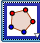
\includegraphics[scale=0.4]{poly.jpg}, construire un carré ABCD.
\item Sélectionner la fenêtre 3D. Une barre, d'icônes propre 3D s'initialise à la place de la barre d'icônes 2D. 


\includegraphics[scale=0.5]{outils-3D.jpg} 

\item Utiliser l'icône 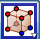
\includegraphics[scale=0.5]{cube.jpg} pour extruder le cube. Cliquer sur les points $A$ et $B$ dans la fenêtre 3D. Et voilà le cube.

On peut placer directement 2 points dans la \textbf{fenêtre 3D }et créer un cube mais si l'on souhaite un cube "posé", il est préférable d'utiliser cette méthode.

\end{enumerate}

\item  Construction d'un plan  

Un plan passe par 3 points non alignés.

 A l'aide de l'icône \textbf{Plan passant par 3 points} 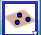
\includegraphics[scale=0.4]{plan.jpg}, construire le plan ABE.
 
\textbf{Attention}, les points induits de la construction du solide construit précédemment ne sont pas sélectionnables \mbox{directement}. Il faut les sélectionner dans la fenêtre \textbf{Algèbre}.

\end{enumerate}


\mini{
\EPCB{1}{GE-3}{ Représenter. Raisonner. Communiquer. }

\EPCB{1}{GE-4}{ Représenter. Raisonner. Communiquer.}

\EPCB{1}{GE-17}{ Modéliser. Calculer. }
}{
\EPCB{1}{GE-5}{ Représenter. Raisonner. Communiquer.}

\EPCB{1}{GE-11}{ Représenter. Raisonner. Communiquer.}

\EPCB{1}{GE-16}{ Représenter. Calculer. Communiquer.}

\EPCNA{Pour aller plus loin}

\url{http://lycee-valin.fr/maths/exercices_en_ligne/espace.html}

}
